\chapter{Frontend electronic of the scintillating fiber hodoscope}\label{cha:frontend}
%the sidevieve hast to be updates
%citroc picute has to be included ans described witharrowas and refreces to the figure have to be included in the text
%slow shaper fater then fast shaper
%table of slow control register has to be checked
%DAC output voltage (\SI{5}{\volt}) has to be understood
\section{Overview of the frontend electronics}
\begin{figure}[h]
    \centering
    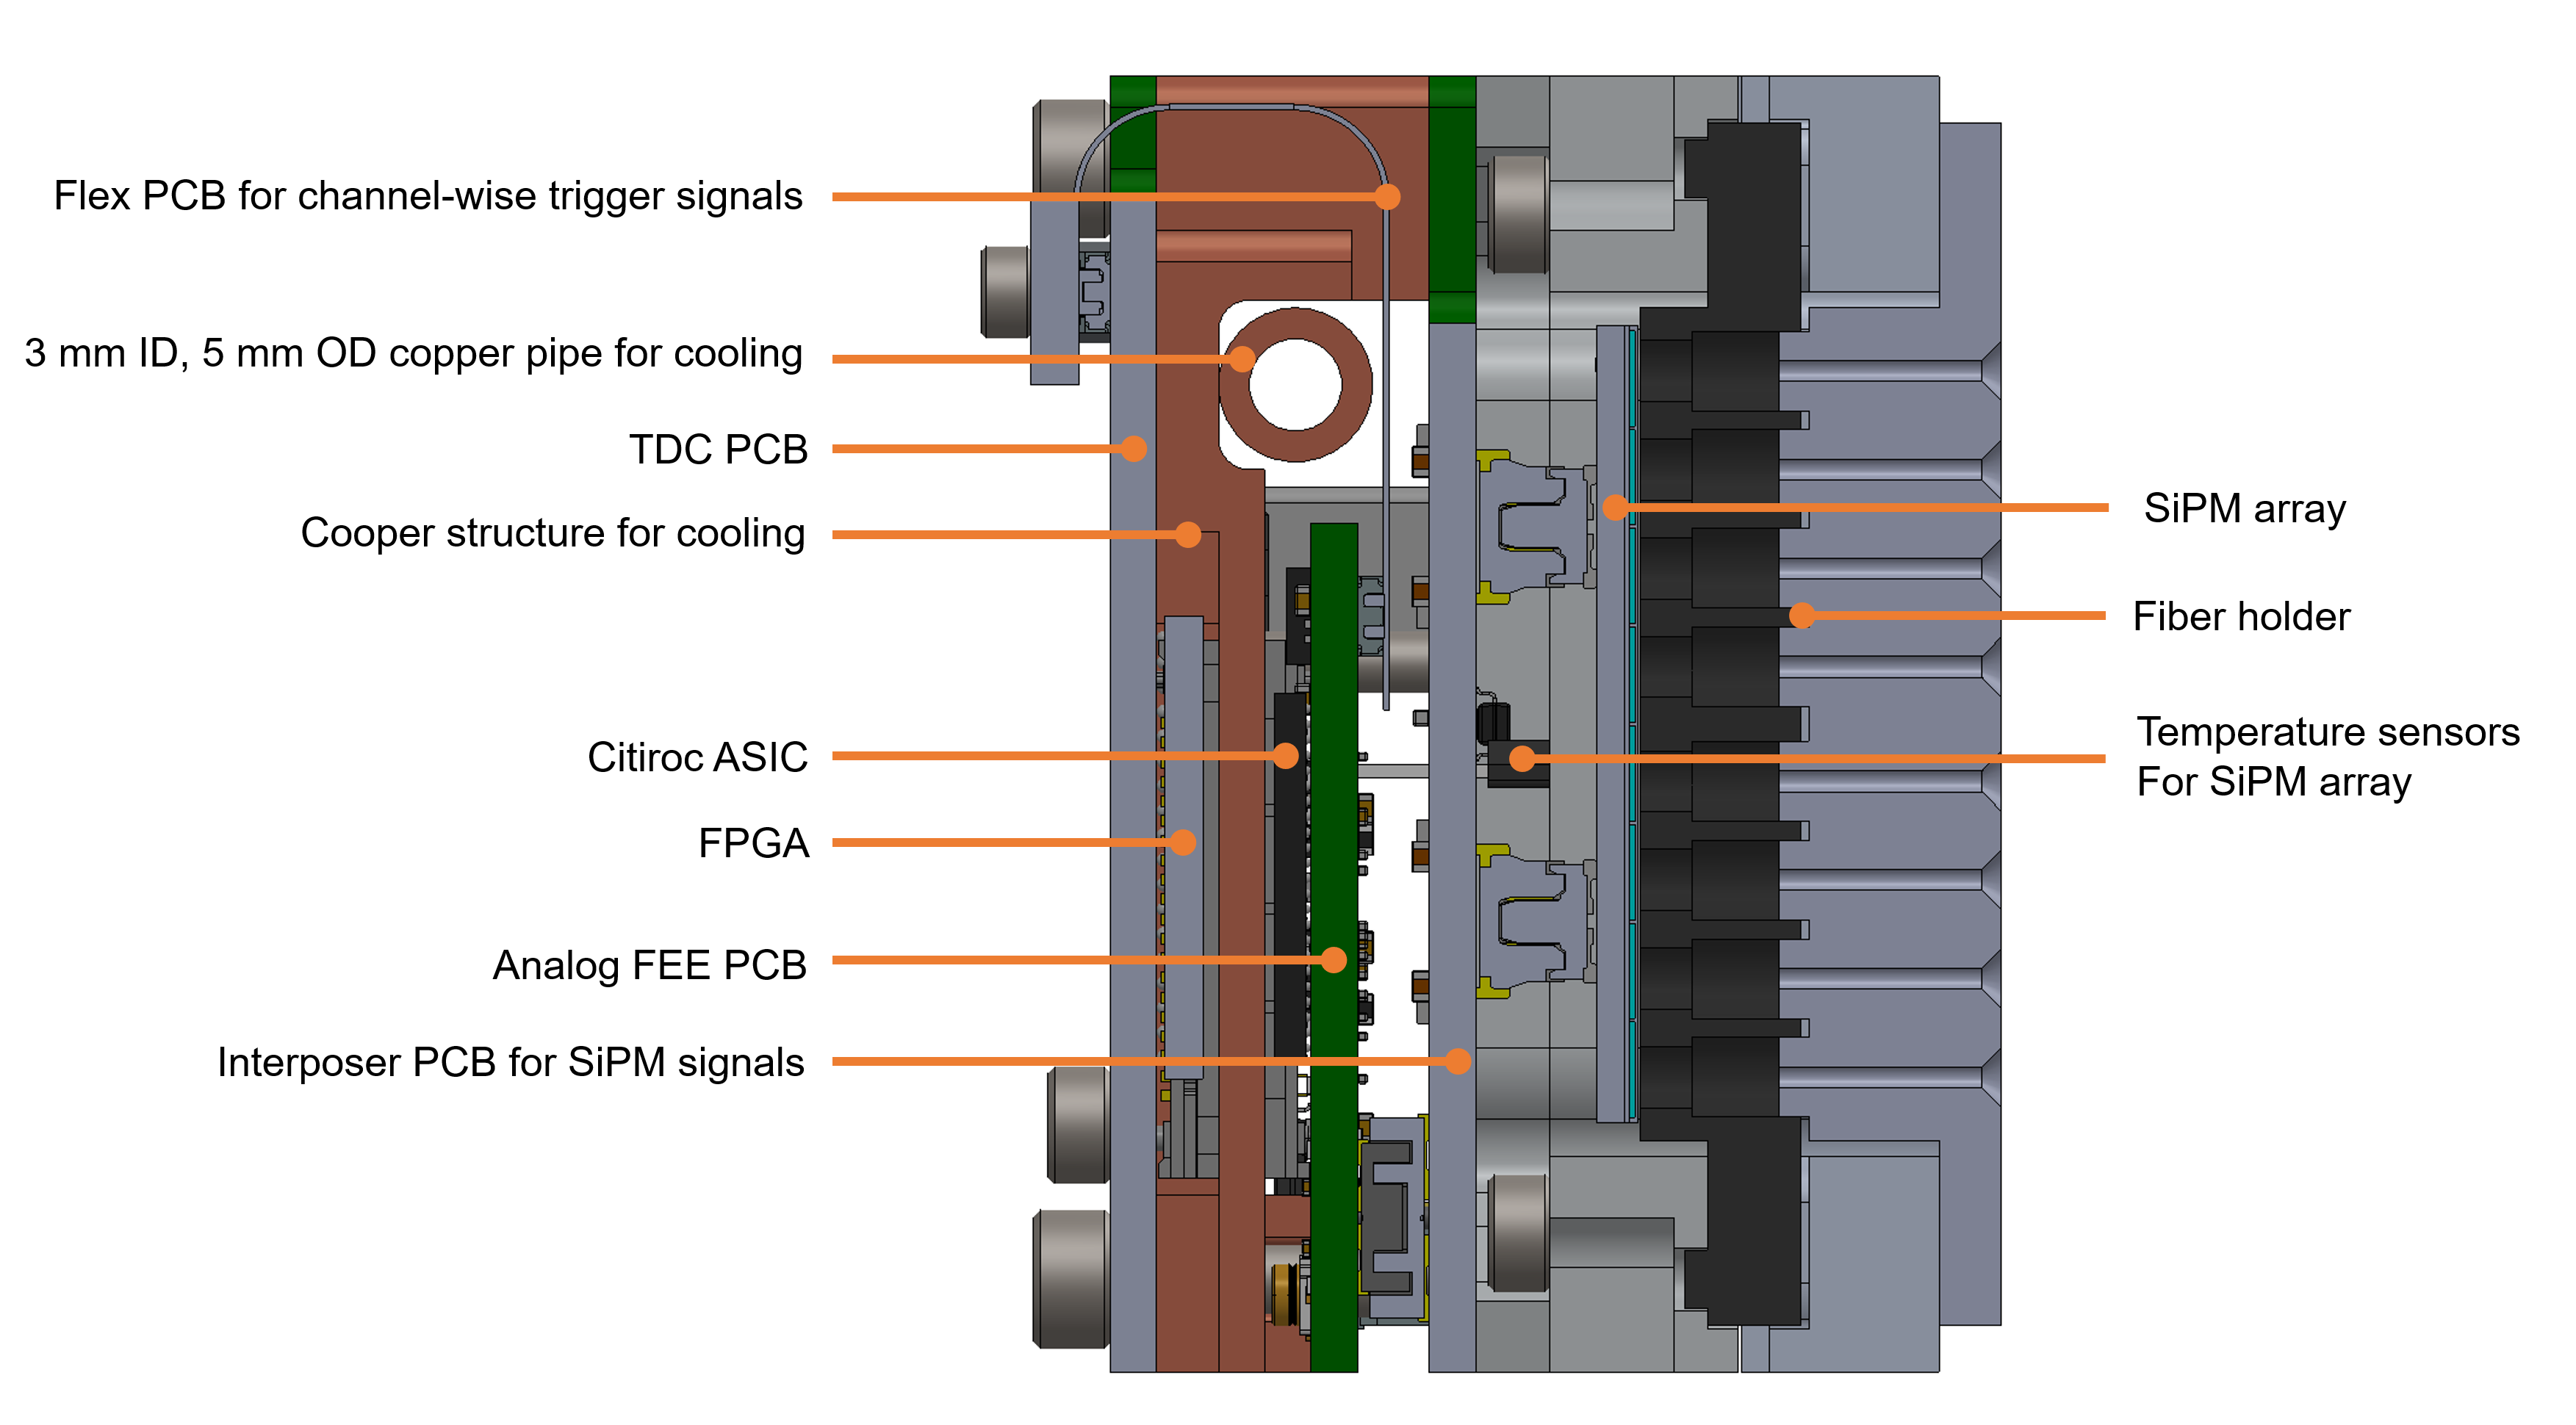
\includegraphics[width=0.9\textwidth]{SideViewElectronics.PNG}
    \caption{Sideview of the frontend electronics that will be attached on the sides of the SFH, the fiber holders will be attached to the fibers.
     The SiPM arrays transform the incoming photons into  electric signals, that are then transferred to the frontend electronics by the PCB interposer.\autocite{InternalcommunicationKarl}}
    \label{fig:SideviewModelElectronics}
    \end{figure}
\subsection{Proccesing of the SFH signal}
The frontend electronics of the scintillating fiber hodoscope process the signals from the scintillating fibers.
They can be attached on all four sides of the SFH, as can be seen in Figure \ref{SFHpicture}.
The fibers are conected to the fiber holders on both ends as shown in Figure \ref{fig:SideviewModelElectronics}. 
There are in total 768\autocite{Amber2022Status} fibers per SFH. Since both ends produce an electric signal,
 a total of 1546 signals or 384 signals, for every attached electonics unit have to be proccesed.
 \newline
 The incoming photons are transformed into electric signals by the SiPM arrays.
 The SiPM signals are then transmitted to the analog frontend electronics (FEE) PCB by the interposer PCB also shown in Figure \ref{fig:SideviewModelElectronics}.\autocite{InternalcommunicationKarl}
\subsection{The analog frontend electronics (FEE) PCB}
\begin{figure}[H]
    \centering
    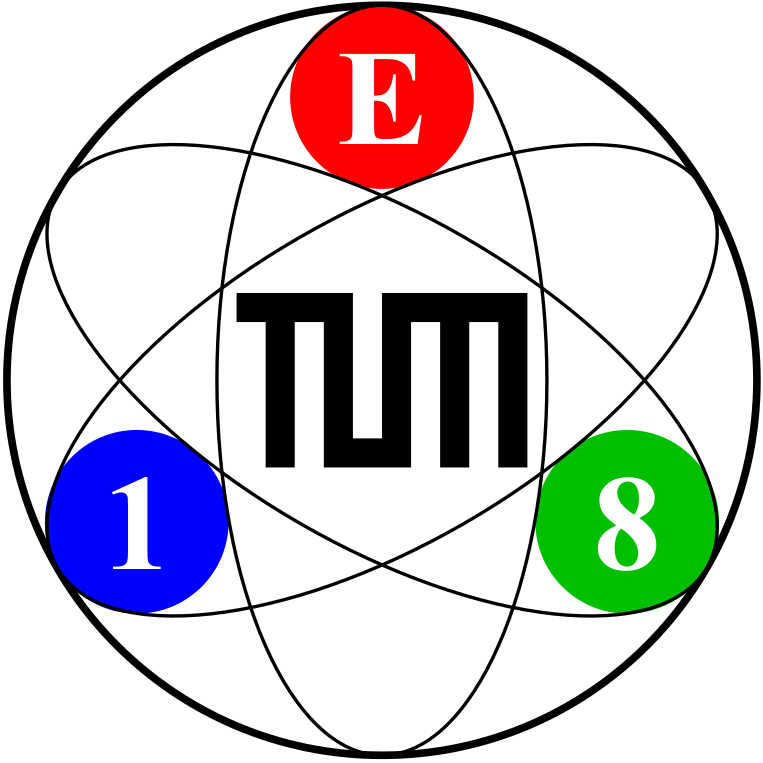
\includegraphics[width=0.6\textwidth]{E18Logo.PNG}
    \caption{The analog frontend electronics (FEE) PCB with the six Citiroc1A ASICs, on the left side the power supply is connected.The output of the Citiroc1A is transmitted to the iFTDC over three flex PCBs.\autocite{InternalcommunicationKarl}}
    \label{fig:FEE}
\end{figure}
The analog frontend electronics (FEE) PCB, shown in Figure \ref{fig:FEE}, together with the iFTDC form the heart of the frontend electronics.
The FEE PCB incorporates six Citiroc1A ASICs, which are designed to amplify and process the signals from the SiPM arrays.
 Each Citiroc1A ASIC handles 32 signals. The output of the Citiroc1A is then transmitted to the iFTDC over three flex PCBs.
The power supply is connected to the FEE PCB on the left side as shown in \ref{fig:FEE}. Two Citirroc1A ASICs are each controlled by one Artix-7 FPGA located on the iFTDC.\autocite{InternalcommunicationIgor}
\subsection{The iFTDC}
\begin{figure}[H]
    \centering
    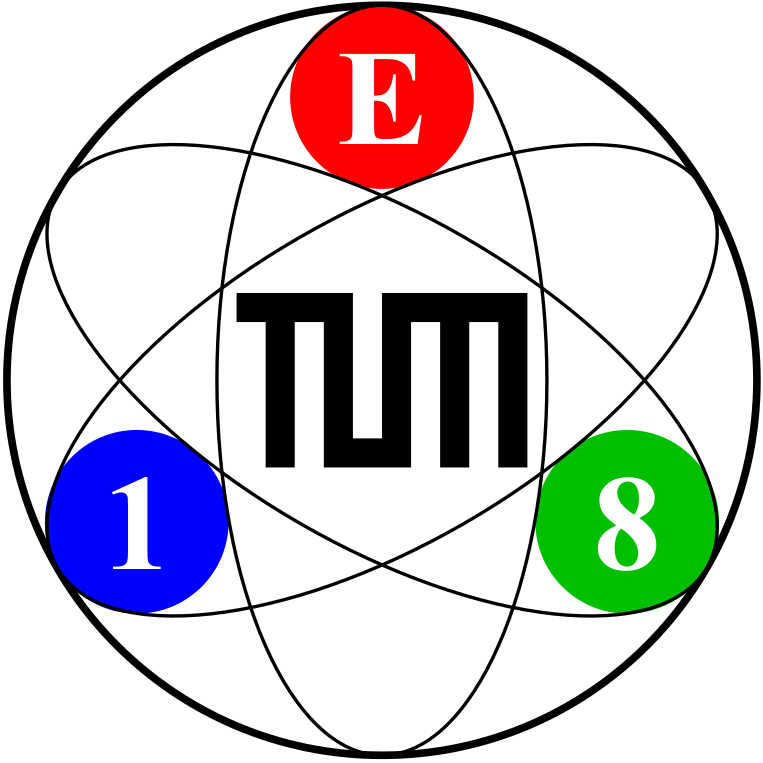
\includegraphics[width=0.6\textwidth]{E18Logo.PNG}
    \caption{The iFTDC with three Artix-7 FPGA, the three flex PCBs that connect the iFTDC with the FEE PCB and the power supply.\autocite{InternalcommunicationIgor}}
    \label{fig:iFTDC}
\end{figure}

The iFTDC, depicted in Figure \ref{fig:iFTDC} is a FPGA based time-to-digital converter. It consists of three Artix-7 FPGA, who each control two Citiroc1A ASICs.
The FPGA handels the readout as well as the configuration of the Citiroc1A ASICs\autocite{InternalcommunicationIgor}.
\newline
INSERT: here stil hast to be includes how ethernet works how ipbus works and how jtag is implemented ans stuff analong this line 
\section{The Citiroc1A ASIC}
The Citiroc1A ASIC is a frontend application-specific integrated circuit developed by Weeroc for the readout of SiPM detectors.
It allows for the readout of 32 channels and is sensitive to $\frac{1}{3}$ of a photoelectron.\autocite{datasheetCITIROC}
\newline
The Citiroc1A ASIC is controlled and readout by the Artix-7 FPGA on the iFTDC, each FPGA controlling two Citiroc1A ASICs.\autocite{InternalcommunicationIgor}
The focus of this thesis is the development of the FPGA firmware for the control of the Citiroc1A ASICs,
 but a provesional readout firmware for testing the configuration of the Citiroc1A will also be developed.
\subsection{Signal proccesing of the Citiroc1A}
\begin{figure}[h]
    \centering
    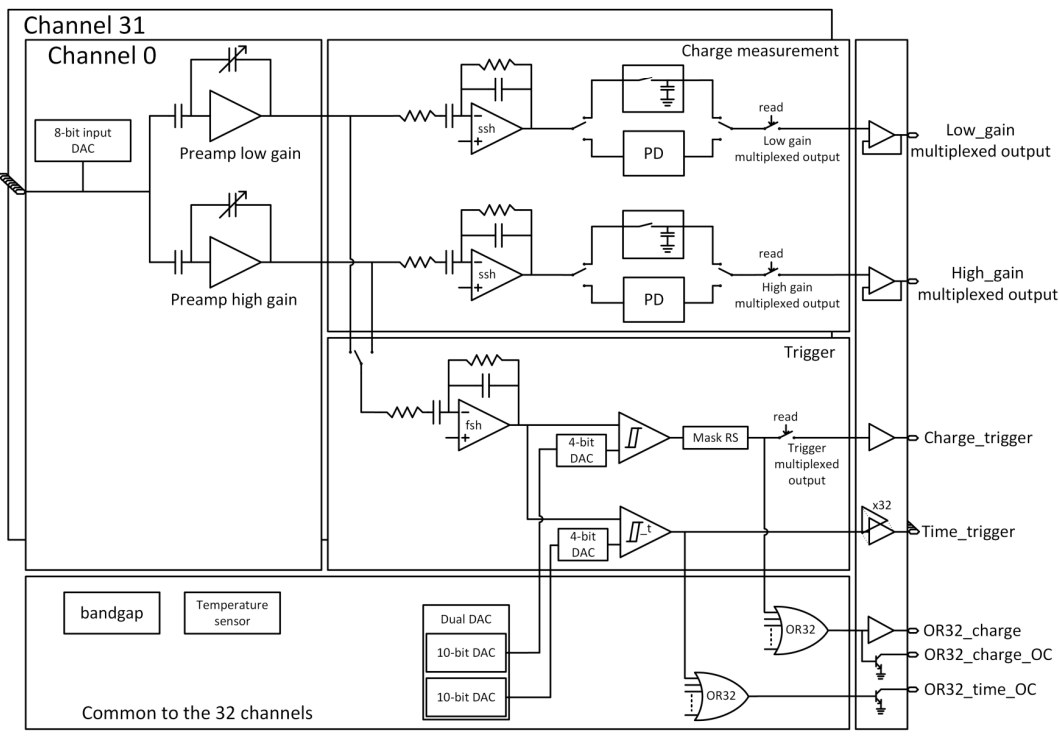
\includegraphics[width=0.8\textwidth]{TRIGER.PNG}
    \caption{General ASIC block scheme of the Citiroc1A. \autocite{datasheetCITIROC}}
    \label{fig:CITIROC1A_TRIGEER}
\end{figure}

\begin{figure}[h]
    \centering
    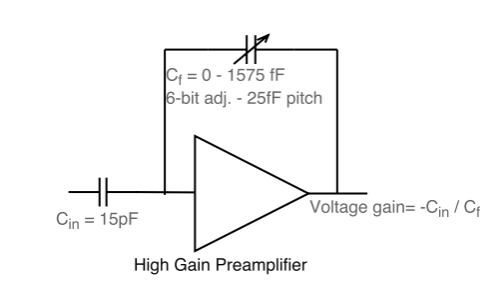
\includegraphics[width=0.8\textwidth]{HighGain.PNG}
    \caption{High gain amplification of the Citiroc1A. The gain is adjustable from 0 to \SI{1575}{\femto\farad} in \SI{25}{\femto\farad} steps.\autocite{datasheetCITIROC}}
    \label{HighGain}
\end{figure}
The general block scheme of the Citiroc1A is shown in Figure \ref{fig:CITIROC1A_TRIGEER}.
\newline
The Citiroc1A allows for the fine tuning of the SiPM bias voltage for each channel via the 8-bit input DAC.
\newline	
The input signals are amplified with a variable high or low gain, configurable for every channel as depicted in Figure \ref{HighGain}. 
The PRM experiment requires the maximal high gain of 62.\autocite{InternalcommunicationIgor}
\newline
The amplified signals are then shaped by either the slow (ssh) or fast shaper (fsh) as shown in Figure \ref{fig:CITIROC1A_TRIGEER}. 
The fast shaper is used for the PRM experiment, since it has a \SI{15}{\nano\second} peaking time, which is needed for the time precision of the SFH.
\newline
The ASIC has two discriminators, the charge discriminator and the time discriminator. In this thesis we will only look at the time discriminator,
 since it provides the time information.
The time discriminator threshold is adjustable via a 10 bit dac for all channels and an additional 4 bit dac for every individual channel as shown in Figure \ref{fig:CITIROC1A_TRIGEER} \autocite{datasheetCITIROC}.


\section{Configuration of the Citiroc1A}
\begin{figure}[h]
    \centering
    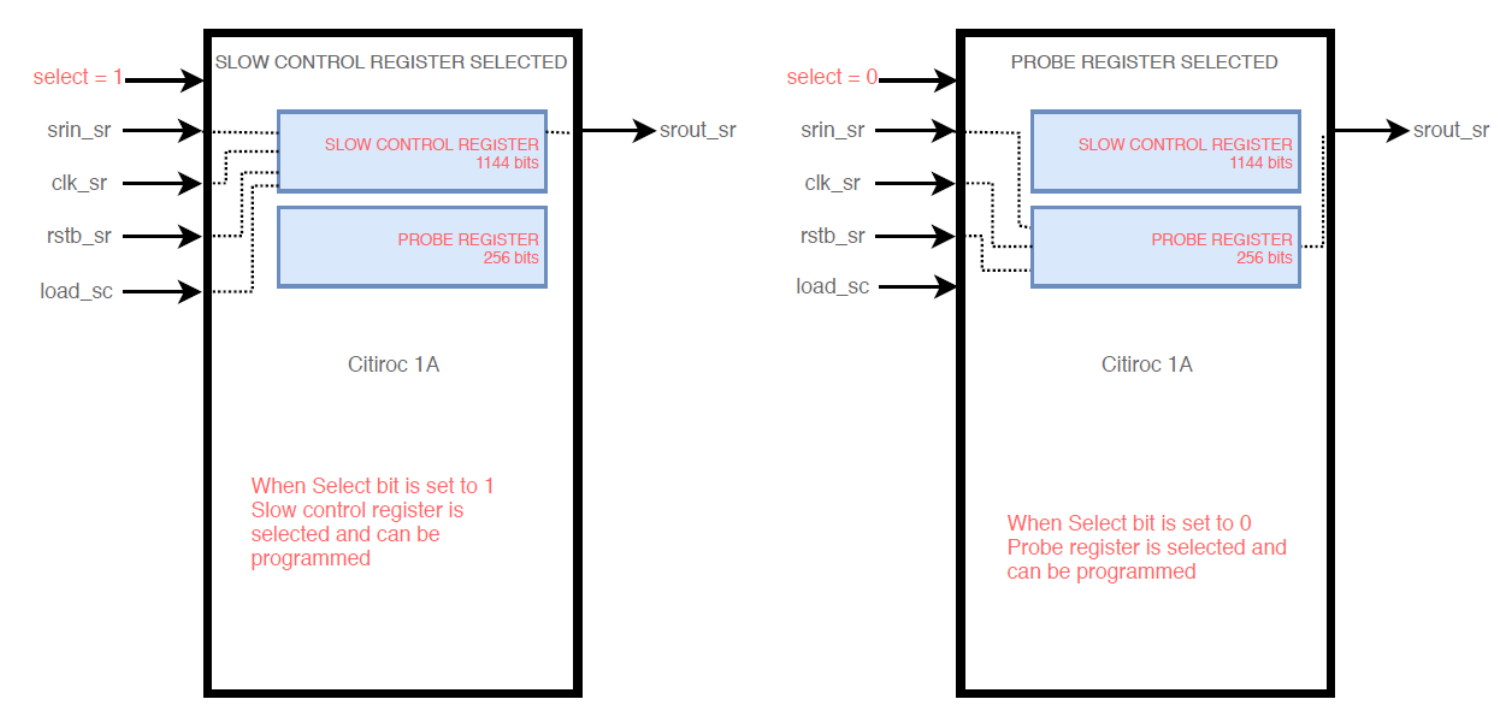
\includegraphics[width=0.8\textwidth]{CitirocConfigHighqual.png}
    \caption{BLABLABLUB\autocite{datasheetCITIROC}}
    \label{fig:CITIROC1A_config}
\end{figure}
The configuration of the Citiroc1A is achievied by the FPGA via the five signals shown in Figure \ref{fig:CITIROC1A_config}.
The SELECT signal allowes the choice between configuring the slow control, for SELECT = 1  or the probe register, for SELECT = 0.\autocite{datasheetCITIROC}

\subsection{The slow control register}

\begin{figure}
    \centering
    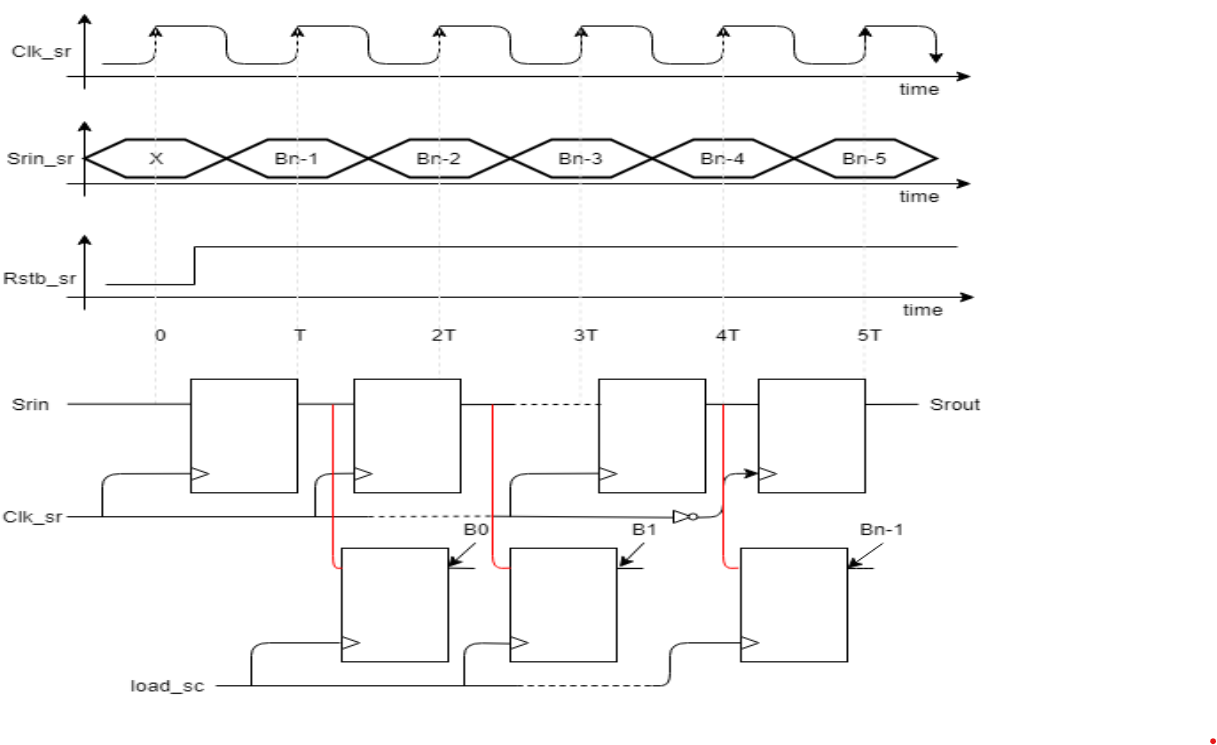
\includegraphics[width=0.8\textwidth]{BitwriteSlowControl.png}
    \caption{BLABLABLUB\autocite{datasheetCITIROC}}
    \label{fig:CITIROC1A_writing_bitstream}
\end{figure}
The slow control register is used to set values for internal variables like the high gain for a channel or the time discriminator threshold.
It also allowes for the FPGA to turn of spesific stages of the Citiroc1A, like the slow shaper or the time discriminator.
The register is 1144 bits long, a full list of all the register that can be set is shown in table \ref{tab:slow_control_register}.
\newline
The process of writing the bitstream into the slow control register by the FPGA is illustrated in Figure \ref{fig:CITIROC1A_writing_bitstream}.


\begin{longtable}{|p{6cm}|p{1cm}|p{1.4cm}|p{1.8cm}|p{5cm}|}
    
    \caption{Configurable registers of the slow control register\autocite{InternalcommunicationKarl} \label{tab:slow_control_register}} \\ \hline
    \hline
\textbf{Register} & \textbf{Bits} & \textbf{Default} & \textbf{Position} & \textbf{Description} \\ \hline
\endfirsthead

\hline
\textbf{Register} & \textbf{Bits} & \textbf{Default} & \textbf{Position } & \textbf{Description} \\ \hline
\endhead

\hline
\multicolumn{5}{r}{{Configurable registers of the slow control register continued on next page}} \\
\endfoot

\hline
\endlastfoot

% channel_thr_time
channel\_thr\_time ch\_0       & 4  & 0 & 0   & Channel-dependent 4-bit threshold for time discriminator. \\ \hline
\multicolumn{5}{|l|}{\emph{See below for common 10-bit threshold.}} \\ \hline
channel\_thr\_time ch\_31      & 4  & 0 & -   & - \\ \hline

% channel_thr_charge
channel\_thr\_charge ch\_0     & 4  & 0 & 128 & Channel-dependent 4-bit threshold for charge discriminator. \\ \hline
\multicolumn{5}{|l|}{\emph{See below for common 10-bit threshold.}} \\ \hline
channel\_thr\_charge ch\_31    & 4  & 0 & -   & - \\ \hline

% discriminator_power
discriminator\_charge\_en      & 1  & 0 & 256 & Enable charge discriminator. \\ \hline
discriminator\_charge\_pp      & 1  & 0 & -   & Power pulse for charge discriminator. \\ \hline
discriminator\_latched\_output & 1  & 0 & -   & 1: latched, 0: direct output. \\ \hline
discriminator\_time\_en        & 1  & 1 & -   & Enable time discriminator. \\ \hline
discriminator\_time\_pp        & 1  & 1 & -   & Power pulse for time discriminator. \\ \hline

% 4-bit DAC settings
4bit\_dac\_charge\_en          & 1  & 0 & 261   & Enable 4-bit charge DAC. \\ \hline
4bit\_dac\_charge\_pp          & 1  & 0 & -   & Power pulse for 4-bit charge DAC. \\ \hline
4bit\_dac\_time\_en            & 1  & 1 & -   & Enable 4-bit time DAC. \\ \hline
4bit\_dac\_time\_pp            & 1  & 1 & -   & Power pulse for 4-bit time DAC. \\ \hline

% channel_discriminator_mask
channel\_discriminator\_mask ch\_0 & 1  & 1 & 265 & 0: masked, 1: unmasked. \\ \hline
\multicolumn{5}{|l|}{\emph{...}} \\ \hline
channel\_discriminator\_mask ch\_31 & 1  & 1 & - & - \\ \hline

% track_and_hold_power
track\_and\_hold\_power high\_gain\_pp & 1  & 0 & 297 & Enable high gain. \\ \hline
track\_and\_hold\_power high\_gain\_en & 1  & 0 & -   & - \\ \hline
track\_and\_hold\_power low\_gain\_pp  & 1  & 0 & -   & Power pulse for low gain. \\ \hline
track\_and\_hold\_power low\_gain\_en  & 1  & 0 & -   & Enable low gain. \\ \hline
track\_and\_hold\_power weak\_bias     & 1  & 0 & -   & 1: weak bias (600kHz max), 0: high bias (5MHz max). \\ \hline

% peak_detector_power
peak\_detector\_power high\_gain\_pp & 1  & 0 & 302 & Enable high gain for peak detector. \\ \hline
peak\_detector\_power high\_gain\_en & 1  & 0 & - & - \\ \hline
peak\_detector\_power low\_gain\_pp  & 1  & 0 & - & Power pulse for low gain. \\ \hline
peak\_detector\_power low\_gain\_en  & 1  & 0 & - & Enable low gain for peak detector. \\ \hline

% select_peak_sensing
select\_peak\_sensing high\_gain\_th & 1  & 0 & 306 & 0: peak detector, 1: track and hold. \\ \hline
select\_peak\_sensing low\_gain\_th  & 1  & 0 & -   & - \\ \hline
peak\_sensing\_cell\_bypass          & 1  & 0 & -   & 0: cell active, 1: bypass peak sensing cell. \\ \hline
peak\_sensing\_external\_trigger     & 1  & 0 & -   & 0: internal trigger, 1: external trigger. \\ \hline

% shaper
shaper fast\_shaper\_follower\_pp & 1  & 0 & 310 & Power pulse for fast shaper follower. \\ \hline
shaper fast\_shaper\_en           & 1  & 1 & -   & Enable fast shaper. \\ \hline
shaper fast\_shaper\_pp           & 1  & 1 & -   & Power pulse for fast shaper. \\ \hline
shaper low\_gain\_slow\_shaper\_pp & 1  & 0 & -   & Power pulse for low gain slow shaper. \\ \hline
shaper low\_gain\_slow\_shaper\_en & 1  & 0 & -   & Enable low gain slow shaper. \\ \hline
shaper low\_gain\_slow\_shaper\_time\_const & 3 & 0 & - & See the table above for values. \\ \hline
shaper high\_gain\_slow\_shaper\_pp & 1 & 0 & - & Power pulse for high gain slow shaper. \\ \hline
shaper high\_gain\_slow\_shaper\_en & 1 & 0 & - & Enable high gain slow shaper. \\ \hline
shaper high\_gain\_slow\_shaper\_time\_const & 3 & 0 & - & See the table above for values. \\ \hline

% (continue for all remaining parameters)
% Preamp Power Settings
low\_gain\_weak\_bias       & 1  & 0 & 323 & 0: normal bias, 1: weak bias. \\ \hline
high\_gain\_pp             & 1  & 1 & -   & Power pulse for high gain preamp. \\ \hline
high\_gain\_en             & 1  & 1 & -   & Enable high gain preamp. \\ \hline
low\_gain\_pp              & 1  & 0 & -   & Power pulse for low gain preamp. \\ \hline
low\_gain\_en              & 1  & 0 & -   & Enable low gain preamp. \\ \hline
fast\_shaper\_low\_gain     & 1  & 0 & -   & 0: fast shaper on high gain. \\ \hline

% Input DAC Settings
dac\_en                   & 1  & 1 & 329 & Input DAC for bias correction. \\ \hline
dac\_ref                  & 1  & 1 & -   & Voltage ref: 1 = internal 4.5V, 0 = internal 2.5V, depends on vdd\_dac. \\ \hline
ch\_0                     & 8  & 255 & - & VSipm = V\_HV - V\_DAC (check what makes sense here). \\ \hline
ch\_0\_en                  & 1  & 1 & -   & Enable channel 0 input DAC. \\ \hline
\multicolumn{5}{|l|}{\emph{...}} \\ \hline
ch\_31                    & 8  & 255 & - & Same as ch\_0 for channel 31. \\ \hline
ch\_31\_en                 & 1  & 1 & -   & Enable channel 31 input DAC. \\ \hline

% Channel Preamp
ch\_0\_hg                  & 6  & 62 & 619 & High gain preamp setting (see Table 3). \\ \hline
ch\_0\_lg                  & 6  & 0  & -   & Low gain preamp setting. \\ \hline
ch\_0\_ctest\_hg            & 1  & 0  & -   & 1: Connect injection capacitance for test signal. \\ \hline
ch\_0\_ctest\_lg            & 1  & 0  & -   & 1: Connect low gain injection capacitance. \\ \hline
ch\_0\_disable             & 1  & 0  & -   & 1 disables preamp for channel 0. \\ \hline
\multicolumn{5}{|l|}{\emph{...}} \\ \hline

% Service Blocks
temp\_pp                  & 1  & 1 & 999   & Enable power pulse for temperature monitoring. \\ \hline
temp\_en                  & 1  & 1 & -   & Enable temperature monitoring. \\ \hline
band\_gap\_pp              & 1  & 1 & -   & Enable power pulse for band gap reference. \\ \hline
band\_gap\_en              & 1  & 1 & -   & Enable band gap reference. \\ \hline

% Threshold DAC
charge\_dac\_en            & 1  & 0 & 1103 & Enable charge threshold DAC. \\ \hline
charge\_dac\_pp            & 1  & 0 & -   & Power pulse for charge threshold DAC. \\ \hline
time\_dac\_en              & 1  & 1 & -   & Enable time threshold DAC. \\ \hline
time\_dac\_pp              & 1  & 1 & -   & Power pulse for time threshold DAC. \\ \hline
charge\_threshold         & 10 & 0 & -   & Charge threshold value. \\ \hline
time\_threshold           & 10 & - & -   & Time threshold value (e.g., ~200 for 1 cell min, ~250 for 2 cells). \\ \hline

% OTAQ Power
high\_gain\_en             & 1  & 1 & 1127 & Enable high gain for OTAQ. \\ \hline
high\_gain\_pp             & 1  & 1 & -    & Power pulse for high gain OTAQ. \\ \hline
low\_gain\_en              & 1  & 0 & -    & Enable low gain for OTAQ. \\ \hline
low\_gain\_pp              & 1  & 0 & -    & Power pulse for low gain OTAQ. \\ \hline
debug\_probe\_en           & 1  & 1 & -    & Enable debug probe. \\ \hline
debug\_probe\_pp           & 1  & 1 & -    & Power pulse for debug probe. \\ \hline

% Input/Output
output\_buffer\_bias       & 1  & 0 & 1133 & Output OTA buffer bias: 0 = auto bias, 1 = force on. \\ \hline
val\_event\_receiver\_en    & 1  & 1 & -    & Enable validation event receiver. \\ \hline
val\_event\_receiver\_pp    & 1  & 1 & -    & Power pulse for validation event receiver. \\ \hline
raz\_chn\_en               & 1  & 1 & -    & Enable RAZ channel. \\ \hline
raz\_chn\_pp               & 1  & 1 & -    & Power pulse for RAZ channel. \\ \hline
digital\_output\_en        & 1  & 1 & -    & Enable digital multiplexed output. \\ \hline
or32\_output\_en           & 1  & 1 & -    & Enable OR32 output. \\ \hline
or32\_oc\_output\_en        & 1  & 1 & -    & Enable OR32 over-current output. \\ \hline
trigger\_polarity         & 1  & 0 & -    & Trigger polarity: 0 = positive (rising edge), 1 = negative (falling edge). \\ \hline
or32\_t\_oc\_en             & 1  & 1 & -    & Enable OR32 timeout over-current. \\ \hline
32\_triggers\_en           & 1  & 1 & 1144    & Enable 32 triggers. \\ \hline
\end{longtable}


\subsection{The probe register}
\begin{figure}[H]
    \centering
    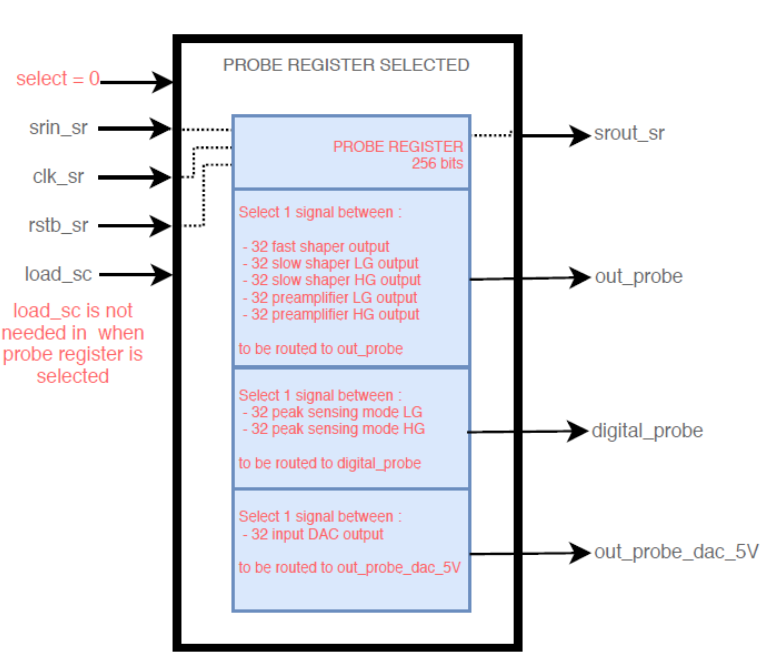
\includegraphics[width=0.8\textwidth]{ProbeRegister.png}
    \caption{BLABLABLUB\autocite{datasheetCITIROC}}
    \label{fig:CITIROC1A_proberegiseter}
\end{figure}
The probe register is used for routing internal signals to several output pins for debugging purposes.
It's functionality is ilustrated in Figure \ref{fig:CITIROC1A_proberegiseter}.
The register consists of 256 bits and is written similarly to the slow control register,
 with the difference that the bits are directly written into the Citiroc1A without requiring a rising edge on load\_sc.
\newline
The internal signals for each channel that can be routed to the output pins are shown in table \ref{tab:probe_register}. 
 \begin{table}[h!]
    \centering
    \begin{tabular}{@{}lll@{}}
    \toprule
    \textbf{Signal Source} & \textbf{Description}                   & \textbf{Output Pin}        \\ \midrule
    High and low gain preamplifier, & Outputs of preamplifiers and shapers & \texttt{out\_probe}        \\
    slow and fast shapers                                                   &                          \\ \midrule
    \texttt{PeakSensing\_modeb\_LG} & Internal peak-sensing signal for low gain & \texttt{digital\_probe}    \\
    \texttt{PeakSensing\_modeb\_HG} & Internal peak-sensing signal for high gain & -    \\ \midrule
    Output of input DAC            & DAC output voltage (\SI{5}{\volt})  & \texttt{out\_probe\_dac\_5\_V} \\ \bottomrule
    \end{tabular}
    \caption{Internal signal routing to output pins for each channel.}
    \label{tab:probe_register}
\end{table}
\newline
Only one signal source can be routed to one output pin at a time, without potentially causing a short circuit.








 

